%%
%% This is file `sample-acmlarge.tex',
%% generated with the docstrip utility.
%%
%% The original source files were:
%%
%% samples.dtx  (with options: `all,journal,bibtex,acmlarge')
%% 
%% IMPORTANT NOTICE:
%% 
%% For the copyright see the source file.
%% 
%% Any modified versions of this file must be renamed
%% with new filenames distinct from sample-acmlarge.tex.
%% 
%% For distribution of the original source see the terms
%% for copying and modification in the file samples.dtx.
%% 
%% This generated file may be distributed as long as the
%% original source files, as listed above, are part of the
%% same distribution. (The sources need not necessarily be
%% in the same archive or directory.)
%%
%%
%% Commands for TeXCount
%TC:macro \cite [option:text,text]
%TC:macro \citep [option:text,text]
%TC:macro \citet [option:text,text]
%TC:envir table 0 1
%TC:envir table* 0 1
%TC:envir tabular [ignore] word
%TC:envir displaymath 0 word
%TC:envir math 0 word
%TC:envir comment 0 0
%%
%% The first command in your LaTeX source must be the \documentclass
%% command.
%%
%% For submission and review of your manuscript please change the
%% command to \documentclass[manuscript, screen, review]{acmart}.
%%
%% When submitting camera ready or to TAPS, please change the command
%% to \documentclass[sigconf]{acmart} or whichever template is required
%% for your publication.
%%
%%
\documentclass[acmlarge]{acmart}
%%
%% \BibTeX command to typeset BibTeX logo in the docs
\AtBeginDocument{%
  \providecommand\BibTeX{{%
    Bib\TeX}}}

%% Rights management information.  This information is sent to you
%% when you complete the rights form.  These commands have SAMPLE
%% values in them; it is your responsibility as an author to replace
%% the commands and values with those provided to you when you
%% complete the rights form.
\setcopyright{acmlicensed}
\copyrightyear{2025}
\acmYear{2025}
\acmDOI{XXXXXXX.XXXXXXX}

%%
%% These commands are for a JOURNAL article.
% \acmJournal{POMACS}
% \acmVolume{37}
% \acmNumber{4}
% \acmArticle{111}
\acmMonth{3}


\usepackage{natbib}
\usepackage{booktabs}
\usepackage{subcaption}
\usepackage{graphicx}
\usepackage{xcolor}
\usepackage{tikz}  % in your preamble
%%
%% Submission ID.
%% Use this when submitting an article to a sponsored event. You'll
%% receive a unique submission ID from the organizers
%% of the event, and this ID should be used as the parameter to this command.
%%\acmSubmissionID{123-A56-BU3}

%%
%% For managing citations, it is recommended to use bibliography
%% files in BibTeX format.
%%
%% You can then either use BibTeX with the ACM-Reference-Format style,
%% or BibLaTeX with the acmnumeric or acmauthoryear sytles, that include
%% support for advanced citation of software artefact from the
%% biblatex-software package, also separately available on CTAN.
%%
%% Look at the sample-*-biblatex.tex files for templates showcasing
%% the biblatex styles.
%%

%%
%% The majority of ACM publications use numbered citations and
%% references.  The command \citestyle{authoryear} switches to the
%% "author year" style.
%%
%% If you are preparing content for an event
%% sponsored by ACM SIGGRAPH, you must use the "author year" style of
%% citations and references.
%% Uncommenting
%% the next command will enable that style.
%%\citestyle{acmauthoryear}


%%
%% end of the preamble, start of the body of the document source.
\begin{document}

%%
%% The "title" command has an optional parameter,
%% allowing the author to define a "short title" to be used in page headers.
\title{Rosys Wizards Multimodal Spell Casting}

%%
%% The "author" command and its associated commands are used to define
%% the authors and their affiliations.
%% Of note is the shared affiliation of the first two authors, and the
%% "authornote" and "authornotemark" commands
%% used to denote shared contribution to the research.
\author{Rose Ordway}
\email{cosyrosy@colostate.edu}

\begin{abstract}
 (Write Abstract Here)
\end{abstract}

%%
%% The code below is generated by the tool at http://dl.acm.org/ccs.cfm.
%% Please copy and paste the code instead of the example below.
%%
\begin{CCSXML}
\end{CCSXML}

% \ccsdesc[500]{Do Not Use This Code~Generate the Correct Terms for Your Paper}
% \ccsdesc[300]{Do Not Use This Code~Generate the Correct Terms for Your Paper}
% \ccsdesc{Do Not Use This Code~Generate the Correct Terms for Your Paper}
% \ccsdesc[100]{Do Not Use This Code~Generate the Correct Terms for Your Paper}

%%
%% Keywords. The author(s) should pick words that accurately describe
%% the work being presented. Separate the keywords with commas.
% \keywords{Do, Not, Us, This, Code, Put, the, Correct, Terms, for,
%   Your, Paper}

% \received{20 February 2007}
% \received[revised]{12 March 2009}
% \received[accepted]{5 June 2009}

%%
%% This command processes the author and affiliation and title
%% information and builds the first part of the formatted document.
\maketitle 

\section{Introduction}
Recently, gesture tracking has seen considerable advancements, which have allowed the creation of new digital experiences that utilize that technology. Meta has been an innovator in their field with their Oculus Quest technology. In 2023, Meta introduced Hand Tracking 2.1 \cite{MetaDevelopers_2023}, which improved the technology. Although hand tracking technology was present in the original Meta Quest, Meta Quest 2, incorporating the 2.1 update of hand tracking, had significant improvements in the accuracy and latency of hand gestures. [more]

Since the release of the 2.1 hand tracking technology, many projects have explored the ideas of hand tracking inputs compared to controller-based inputs. Darkheir, launched on May 8, 2023, is a full hand-tracking VR game that uses a lot of the systems made possible with the 2.1 Hand Tracking system. Other researchers, such as Khundam, have conducted comparative studies on the differences between controllers and hand tracking. These pursuits show an interest in hand tracking vs. controller interactivity to create better user experiences.

The objective of this project is to create a VR spell-based casting system that utilizes gestures and controller inputs. These control systems will be compared to determine which is the most effective and user-friendly. We will conduct experiments on the accuracy, user satisfaction, and completion time of control systems. VR is inherently about the development of immersive experiences, and knowing the most intuitive and pleasant aspects of the user experience will enhance immersion in an experience. This project aims to identify a more immersive method of interacting with the digital space by using the Meta Quest 3 hand tracking technology, which has advanced from hand tracking 2.1 to Hands 2.3\cite{Meta_2024}.


% \begin{table}
%   \caption{Frequency of Special Characters}
%   \label{tab:freq}
%   \begin{tabular}{ccl}
%     \toprule
%     Non-English or Math&Frequency&Comments\\
%     \midrule
%     \O & 1 in 1,000& For Swedish names\\
%     $\pi$ & 1 in 5& Common in math\\
%     \$ & 4 in 5 & Used in business\\
%     $\Psi^2_1$ & 1 in 40,000& Unexplained usage\\
%   \bottomrule
% \end{tabular}
% \end{table}



% \begin{table*}
%   \caption{Some Typical Commands}
%   \label{tab:commands}
%   \begin{tabular}{ccl}
%     \toprule
%     Command &A Number & Comments\\
%     \midrule
%     \texttt{{\char'134}author} & 100& Author \\
%     \texttt{{\char'134}table}& 300 & For tables\\
%     \texttt{{\char'134}table*}& 400& For wider tables\\
%     \bottomrule
%   \end{tabular}
% \end{table*}

\section{Related Works}
There have been several research projects and games that have used gesture controls to explore new interaction techniques with VR. An example of these games is Darkheir \cite{HXDF_2025}, which champions itself as the "Fist Hand Tracking ARPG." One thing a system like Darkheir's hand tracking will always struggle with is providing adequate spell feedback to the user. Haptics in the controller give a responsive feeling to any interaction happening in the digital world. This means that if an experience or game needs to be fully hand-tracking, the feedback from audio and visual content needs to be as responsive and unambiguous as possible. While this game does an impressive job of showing off what can be accomplished using the hand-tracking systems of the Meta Quest, it might not be the most efficient or user-friendly way of creating or interacting with digital spells. 

While there have been studies on comparing the best way to introduce people to or provide information in VR with hand tracking or controllers, there does not seem to be any going in-depth on the idea of interacting with a digital space. In a study by Khundam \cite{khundam2021comparative}, they found that comparing VR hand tracking to VR controllers had no effect on the interaction time or enjoyment of users. The study found no significant impact on the interaction time or enjoyment of users.  While the study finds this, it explored intubation training for real-world situations. This might create a bias, as real-world intubation training could be more stressful and dangerous, making the VR space safer. This study is interested in only dealing with digital interaction and the feedback that can be found from that, while the Khundam study focuses on making real-world learning applications easier.

\section{Methodology}
The development of this project will use Unity as its base, as it incorporates the XR Interaction Toolkit, which clearly defines a gesture-based system for creating and tracking events. The XR Interaction Toolkit simplifies a great deal of the code and process to create a functional and testable VR project. New C\# scripts will be built to handle spell and glyph interaction events. Making the entire experience game-driven eliminates the need for the tester to teach project components. Unity also provides an excellent menu system to organize testing options. Because the project investigates the comfortability and compatibility levels of controllers vs. hand gestures, the ability to swap control types is essential as it will speed up testing. We will use XR Interaction's excellent resources for hand gesture implementations to enhance the user's intuitiveness in casting spells.

\subsection{Evaluation and Metrics}
The experiment in this project aims to test the difference between five different methods of trying to cast spells. Each experiment will have the subject try each different input method and complete a "lesson" using that input method. These lessons aim to gather data on speed, error rate, user fatigue, and user enjoyment. We will measure all this data to identify statistically significant user preferences and effectiveness differences.


\noindent
\begin{center}
\begin{table}[ht]
  \centering
  \caption{Input Methods and Their Abbreviations}
  \label{tab:input-abbr}
  \begin{tabular}{@{}ll@{}}
    \toprule
    \textbf{Input Method}                     & \textbf{Abbreviation} \\ 
    \midrule
    Controller One-Handed                     & C1H   \\
    Controller Two-Handed                     & C2H   \\
    Gesture One-Handed                        & G1H   \\
    Gesture Two-Handed Separate               & G2H-S \\
    Gesture Two-Handed Combined               & G2H-C \\
    \bottomrule
  \end{tabular}
\end{table}
\end{center}

These input methods are controller one-handed (C1H), controller two-handed (C2H), gesture one-handed (G1H), separate gesture two-handed (G2H-S), and combined gesture two-handed (G2H-C). Table 1 includes all the abbreviations needed for these input methods. The controller inputs will use the buttons, triggers, and grips to create the inputs required to create a glyph. The gesture input method will use simple gestures to create these game glyphs. The difference between the gesture types, separate and combined, is that separate will be two of the same gesture on two different hands, such as two peace signs or two fists. In comparison, the combined gestures will require two hands to complete, such as heart hands or creating a triangle. The first step of every lesson in the game is to understand what gestures there are and how to use them to create a basic glyph.

Each participant will go through five lessons. Each lesson will cover eight to twelve random spells made from a preselected set of glyphs. We will evaluate each participant on the following criteria:


\begin{table}[ht]
  \centering
  \small
  \caption{Evaluation criteria and their operational definitions}
  \label{tab:evaluation-criteria}
  \begin{tabular}{@{}p{0.28\textwidth}p{0.65\textwidth}@{}}
    \toprule
    \textbf{Criterion} & \textbf{Definition / Metrics} \\
    \midrule
    Glyph Creation Accuracy  
      & Proportion of correctly formed glyphs; record each success/failure. \\[0.5em]
    Time Measurements  
      & 
      \begin{tabular}[t]{@{}l@{}}
      \textbf{Average Time Per Input:} time from prompt to correct button/gesture \\ 
      \textbf{Average Time Per Spell:} time to complete one set of three glyphs \\ 
      \textbf{Per Lesson:} total time to finish all spells in a lesson
      \end{tabular} \\[0.5em]
    User Enjoyment  
      & Self-reported enjoyment (Rated from 1 to 5) \\[0.5em]
    \bottomrule
  \end{tabular}
\end{table}

The system will measure time and accuracy, collecting user gameplay data. The system will input this data into a CSV data sheet to ensure the tester or participant does not bias any user data. After the last lesson, the participant will be asked to rate the control types from 1 to 5, with 1 being the user's favorite, to see if there is any discrepancy between user favorites and user efficiency. We will use all this information to assess the efficiency and enjoyment of each input method.


\section{Results}

\subsection{Participants}
This study recruited 15 people between the ages of 16 and 49, all with varying experience in VR and gaming (4 identified as women and 11 as men, M = 21.46, Mdn = 18), to participate in the study. Table 3 provides complete demographics and VR and gaming experience. Of the participants, seven reported having VR experience, and 12 reported experience with gaming. Sessions were done in indoor settings (e.g., a lab room, classroom, or the participants' home), all under similar conditions.

\subsection{Apparatus and Applications}
The experiment was done using a standalone Meta Quest 3 MHD and utilized a fully within-subject design, as each participant completed all five control types (C1H, C2H, G1H, G2H-S, and G2H-C) in a single session. To balance against the learning curve of the game, we recruited a total number of participants divisible by five, ensuring that each method was able to be first. Some participants took short rest breaks in between the different control types. The goal was that by randomizing and evenly distributing the starting input, the bias from learning or fatigue would not affect the final results.
\begin{table}[ht]
  \centering
  \small  % reduce font size for the table
  \caption{Participant demographics and prior experience}
  \label{tab:participants}
  \begin{tabular}{@{}ccccc@{}}
    \toprule
    \textbf{ID} & \textbf{Age} & \textbf{Gender} & \textbf{VR Experience} & \textbf{Gaming Experience} \\
    \midrule
    P1  & 22 & F & No  & Yes \\
    P2  & 18 & F & No  & No  \\
    P3  & 16 & M & No  & Yes \\
    P4  & 25 & M & Yes & Yes \\
    P5  & 17 & M & Yes & Yes \\
    P6  & 18 & M & No  & Yes \\
    P7  & 18 & F & No  & No  \\
    P8  & 17 & M & Yes & Yes \\
    P9  & 24 & F & No  & Yes \\
    P10 & 18 & M & No  & Yes \\
    P11 & 16 & M & Yes & Yes \\
    P12 & 49 & M & No  & No  \\
    P13 & 16 & M & Yes & Yes \\
    P14 & 24 & M & Yes & Yes \\
    P15 & 24 & M & Yes & Yes \\
    \bottomrule
  \end{tabular}
\end{table}

\subsection{Protocol}
The data for this study was found using a game created in Unity called Rosy's Wizards 465. In the game, users will choose one of the five control types and play through a series of different lessons, including a tutorial lesson, a glyph input lesson, and a final spellcasting lesson. The game aims to cast various spells by creating glyphs using different inputs, including gestures and controllers. The background stats, including their accuracy and time, will be tracked as the user goes through the lessons. The user will determine these correct inputs by following the inputs on the chalkboards before them. The left board is considered the teacher board, which includes all of the information the user needs to accomplish, and the right board is regarded as the student board, which is what the user has inputted. Both boards will give immediate feedback to the user, changing to green or red accordingly. Users will also find a control list board in the center of the two boards, which shows the user the correct assignments for each gesture or input they are doing. This was put here so users would not have to memorize the tutorial's glyph inputs, slowing down testing and making the game harder for users. At the end of the lesson, the user will find a statistics board with all their gameplay statistics over the lessons.




\begin{figure}[ht]
  \centering
  \begin{tikzpicture}
    \node[
      draw=black,             % border color
      line width=1pt,         % border thickness
      rounded corners=3pt,    % slight rounding
      inner sep=5pt           % padding around the image
    ] {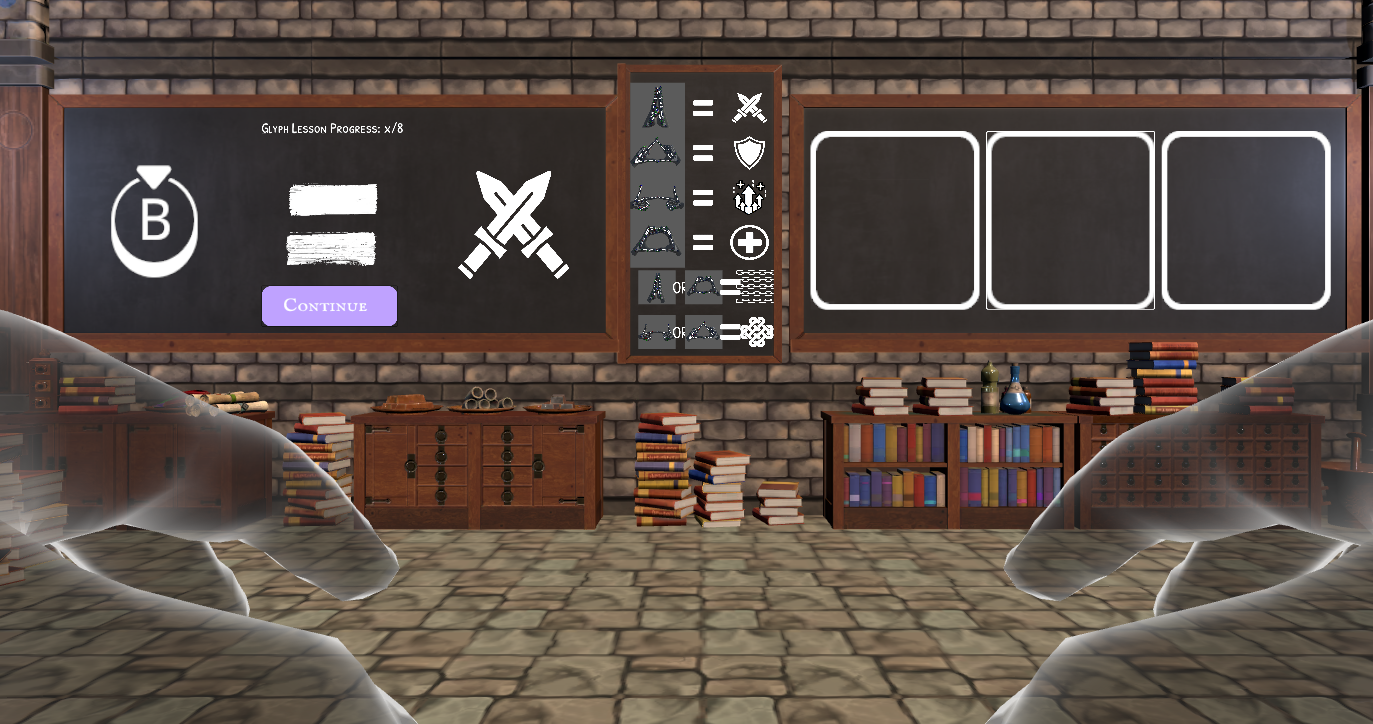
\includegraphics[width=\linewidth]{chalkboards.png}};
  \end{tikzpicture}
  \caption{In-game chalkboard layout in Rose’s Wizard 465. \textbf{Left:} “Teacher” board showing the target glyph sequence and progress indicator. \textbf{Center:} Control mapping board listing the current glyph–input assignments. \textbf{Right:} “Student” board where the user’s inputs appear with immediate green/red feedback.}
  \label{fig:chalkboards}
\end{figure}


\begin{figure}[ht]
  \centering
  % First row: Attack, Defense, Buff
  \begin{subfigure}[t]{0.3\textwidth}
    \centering
    \colorbox{black!100}{
\includegraphics[width=0.6\linewidth]{attack.png}}
    \caption{Attack}
    \label{fig:glyph-attack}
  \end{subfigure}\hfill
  \begin{subfigure}[t]{0.3\textwidth}
    \centering
    \colorbox{black!100}{
\includegraphics[width=0.6\linewidth]{shield-icon-antivirus-icon-png.png}}
    \caption{Defense}
    \label{fig:glyph-defense}
  \end{subfigure}\hfill
  \begin{subfigure}[t]{0.3\textwidth}
    \centering
    \colorbox{black!100}{
\includegraphics[width=0.6\linewidth]{Buff.png}}
    \caption{Buff}
    \label{fig:glyph-buff}
  \end{subfigure}
  
  \vspace{1em}
  
  % Second row: Health, Link, Weave
  \begin{subfigure}[t]{0.3\textwidth}
    \centering
    \colorbox{black!100}{
\includegraphics[width=0.6\linewidth]{Health.png}}
    \caption{Health}
    \label{fig:glyph-health}
  \end{subfigure}\hfill
  \begin{subfigure}[t]{0.3\textwidth}
    \centering
    \colorbox{black!100}{
\includegraphics[width=0.6\linewidth]{Link.png}}
    \caption{Link}
    \label{fig:glyph-link}
  \end{subfigure}\hfill
  \begin{subfigure}[t]{0.3\textwidth}
    \centering
    \colorbox{black!100}{
\includegraphics[width=0.6\linewidth]{Weave.png}}
    \caption{Weave}
    \label{fig:glyph-weave}
  \end{subfigure}

  \caption{Glyph icons for the Rosy’s Wizard lessons: Attack, Defense, Buff, Health, Link, and Weave.}
  \label{fig:glyph-icons}
\end{figure}


\subsection{Lessons}

\subsubsection{Input Lesson}
Participants learn which button or gesture produces each glyph. We record:
\begin{itemize}
  \item \emph{Input accuracy}: proportion of correct inputs
  \item \emph{Average input time}: time from glyph prompt to correct entry
\end{itemize}
Total lesson time is not measured, since input counts vary (e.g.\ G1H requires 8 inputs, G2H only 4).

\subsubsection{Glyph Lesson}
Participants combine glyphs to form spells without feedback. Each trial samples from 32 possible sequences of four glyph types (Attack, Defense, Buff, Heal) and two connectors (Link, Weave). We record:
\begin{itemize}
  \item \emph{Average time to input three glyphs}
  \item \emph{Glyph input accuracy}
  \item \emph{Total completion time} over eight spells (with retries on error)
\end{itemize}

\subsubsection{Spell Lesson}
Participants cast 16 spells with real‐time visual feedback (spell effects and environmental changes) to simulate the final trial. Measures mirror the Glyph Lesson to assess performance under fatigue:
\begin{itemize}
  \item \emph{Average time to input three glyphs}
  \item \emph{Glyph input accuracy}
  \item \emph{Total completion time}
\end{itemize}
\subsubsection{How Spells Were Scored}
\begin{itemize}
      \item \emph{Story Dialogue:}  
        Narrative interludes (“story dialogue”) were excluded from all timing measures but logged to quantify break frequency.  
      \item \emph{Accuracy:}  
        Calculated per lesson as  
        \[
          \mathrm{Accuracy} \;=\; 1 \;-\; \frac{\#\,\text{incorrect inputs}}{\#\,\text{correct inputs} + \#\,\text{incorrect inputs}}
        \]
      \item \emph{Average Input Time:}  
        Measured from when a prompt appears on the teacher board to the moment of the correct input.  
      \item \emph{Lesson Completion Time:}  
        Measured from the first prompt display to the final correct input in each lesson.  
   

\end{itemize}

\subsection{Control Types Tested}

Figure~\ref{fig:control_boards} shows the control‐board layouts for all five control types.  

\begin{figure}[ht]
  \centering
  \makebox[\textwidth][c]{%
    % Five boards at 0.19\textwidth each
    \begin{subfigure}[t]{0.19\textwidth}
      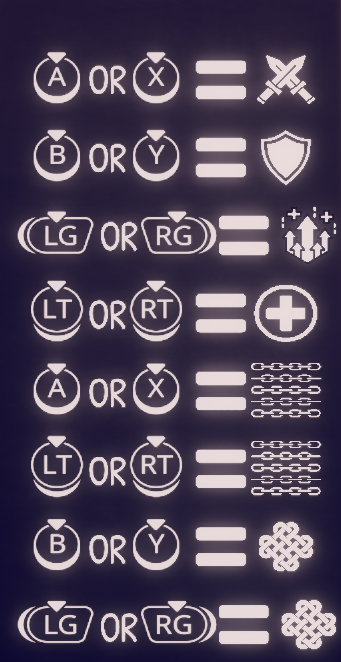
\includegraphics[width=\linewidth]{C1H-Board.png}
      \caption{C1H}
      \label{fig:board-c1h}
    \end{subfigure}\hfill
    \begin{subfigure}[t]{0.19\textwidth}
      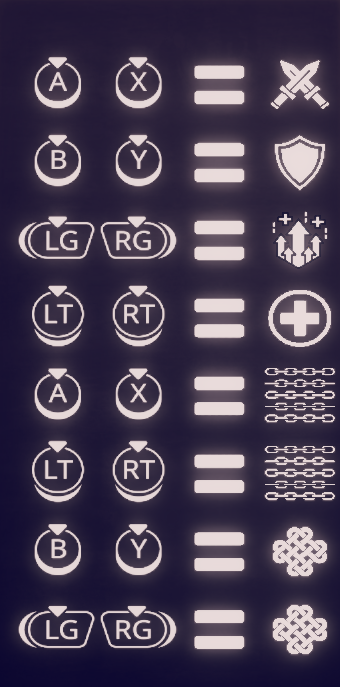
\includegraphics[width=\linewidth]{C2H-Board.png}
      \caption{C2H}
      \label{fig:board-c2h}
    \end{subfigure}\hfill
    \begin{subfigure}[t]{0.19\textwidth}
      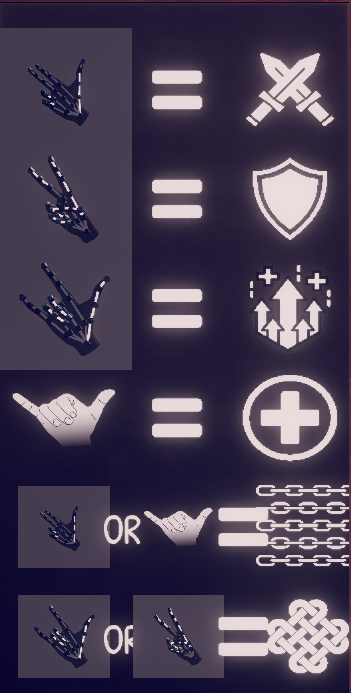
\includegraphics[width=\linewidth]{G1H-Board.png}
      \caption{G1H}
      \label{fig:board-g1h}
    \end{subfigure}\hfill
    \begin{subfigure}[t]{0.19\textwidth}
      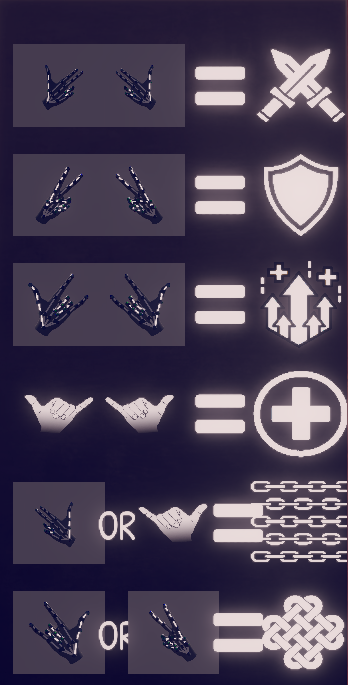
\includegraphics[width=\linewidth]{G2H-Board.png}
      \caption{G2H-S}
      \label{fig:board-g2hs}
    \end{subfigure}\hfill
    \begin{subfigure}[t]{0.19\textwidth}
      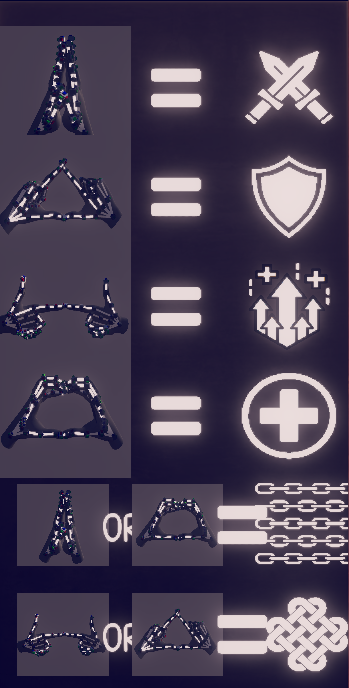
\includegraphics[width=\linewidth]{G2H-C-Board.png}
      \caption{G2H-C}
      \label{fig:board-g2hc}
    \end{subfigure}%
  }
  \caption{Control-list boards for all five input methods in Rose’s Wizard 465.}
  \label{fig:control_boards}
\end{figure}



\begin{table}[ht]
  \centering
  \caption{Glyph–Input mappings for the two controller conditions}
  \label{tab:controller-mappings}
  \begin{tabular}{@{}ll@{\qquad}ll@{}}
    \toprule
    \multicolumn{2}{c}{\textbf{Controller One-Handed (C1H)}}  
      & \multicolumn{2}{c}{\textbf{Controller Two-Handed (C2H)}} \\
    \cmidrule(r){1-2} \cmidrule(l){3-4}
    \textbf{Glyph} & \textbf{Input Mapping (Either Hand) }  
      & \textbf{Glyph} & \textbf{Input Mapping (Two‐Handed)} \\
    \midrule
    Attack   & Primary button 
      & Attack   & Primary buttons   \\
    Defense  & Secondary button 
      & Defense  & Secondary buttons   \\
    Buff     & Grip button  
      & Buff     & Grip buttons \\
    Health   & Trigger button  
      & Health   & Trigger buttons  \\
    Link     & Primary or Trigger   
      & Link     & Primary or Trigger \\
      Weave    & Secondary or Grip  
      & Weave    & Secondary or Grip   \\
    \bottomrule
  \end{tabular}
\end{table}



\begin{figure}[ht]
  \centering
  \begin{subfigure}[t]{0.23\textwidth}
    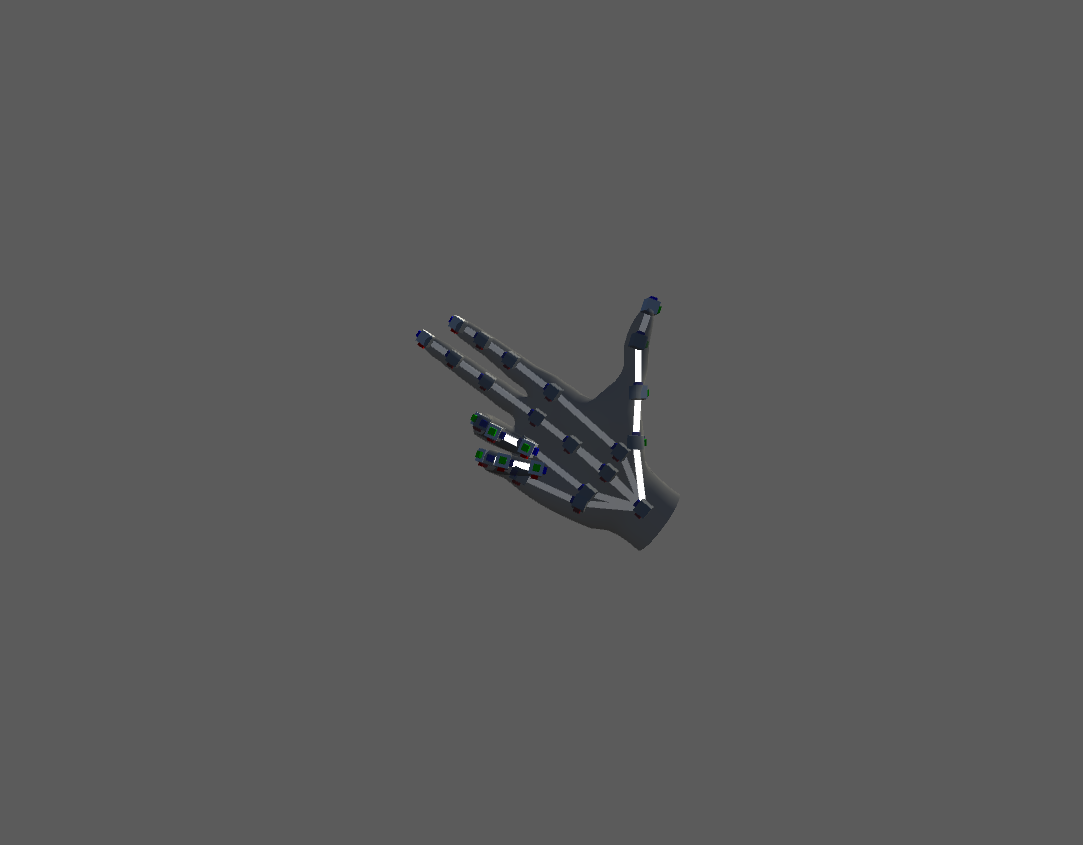
\includegraphics[width=\linewidth]{Finger Guns.png}
    \caption{Finger Guns (Attack)}
    \label{fig:gesture-fingerguns}
  \end{subfigure}\hfill
  \begin{subfigure}[t]{0.23\textwidth}
    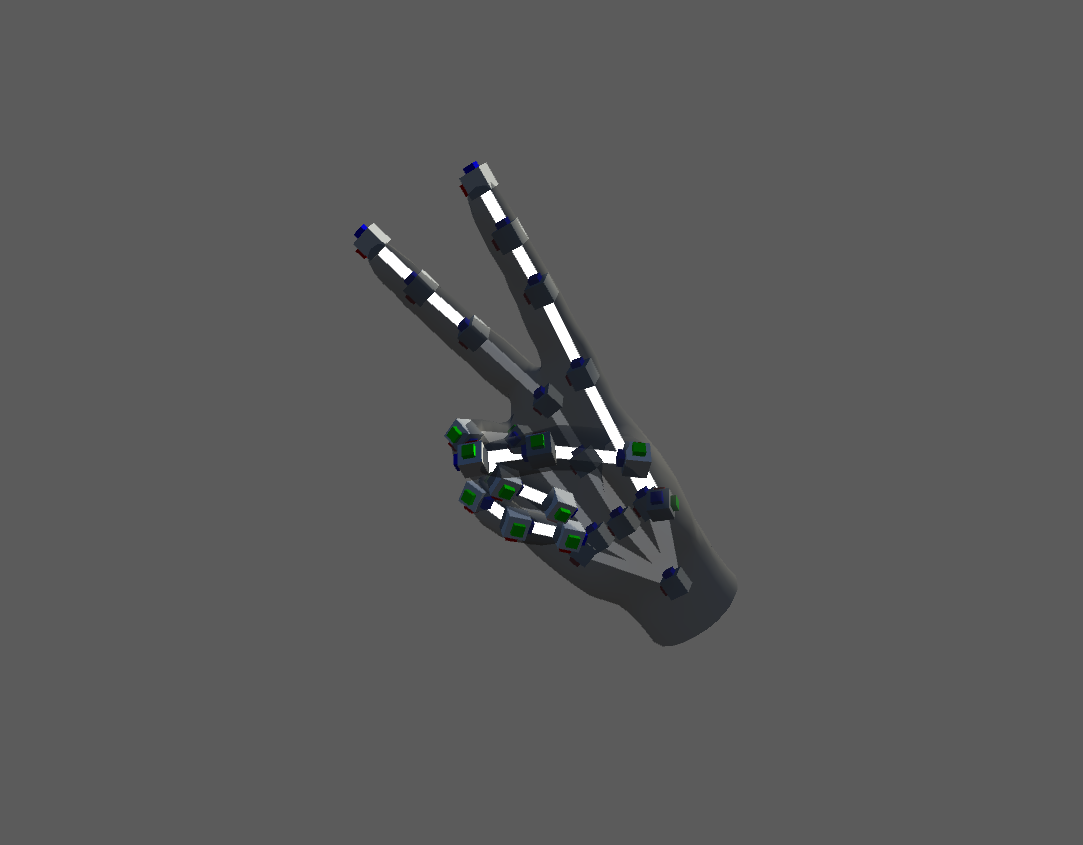
\includegraphics[width=\linewidth]{Peace Sign.png}
    \caption{Peace Sign (Defense)}
    \label{fig:gesture-peacesign}
  \end{subfigure}\hfill
  \begin{subfigure}[t]{0.23\textwidth}
    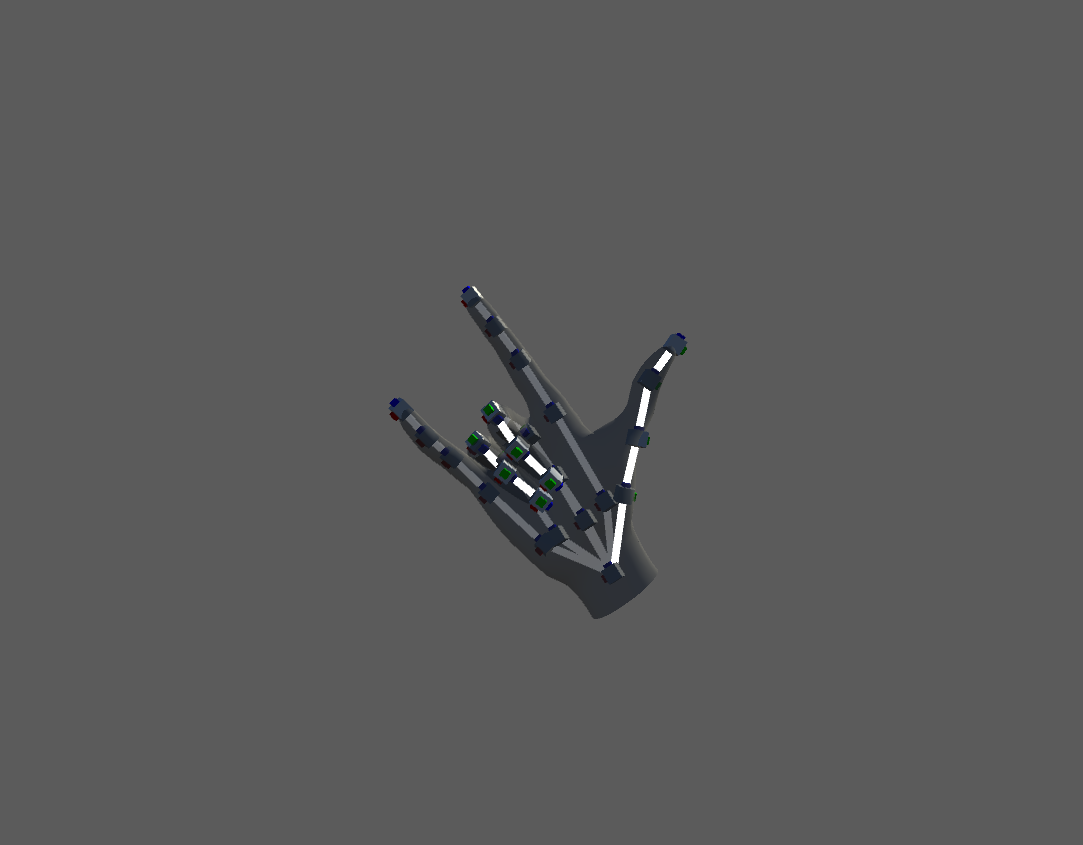
\includegraphics[width=\linewidth]{Rocker.png}
    \caption{Rocker (Buff)}
    \label{fig:gesture-rocker}
  \end{subfigure}\hfill
  \begin{subfigure}[t]{0.23\textwidth}
    
\includegraphics[width=\linewidth]{Shaka.png}
    \caption{Shaka (Health)}
    \label{fig:gesture-shaka}
  \end{subfigure}
  \caption{Gesture–glyph mappings for the one‐handed and two‐handed gesture conditions.}
  \label{fig:gesture-collage}
\end{figure}


\begin{table}[ht]
  \centering
  
  \label{tab:gesture-mappings}
  \begin{tabular}{@{}ll@{\quad}ll@{}}
    \toprule
    \multicolumn{2}{c}{\textbf{Gesture One‐Handed (G1H)}}  
      & \multicolumn{2}{c}{\textbf{Gesture Two‐Handed (G2H)}} \\
    \cmidrule(r){1-2} \cmidrule(l){3-4}
    \textbf{Glyph} & \textbf{Gesture (Either Hand) }  
      & \textbf{Glyph} & \textbf{Gesture (Two‐Handed)} \\
    \midrule
    Attack   & Finger Guns                      & Attack   & Finger Guns  \\
    Defense  & Peace Sign                       & Defense  & Peace Sign \\
    Buff     & Rocker                           & Buff     & Rocker  \\
    Health   & Shakka                           & Health   & Shakka  \\
    Link     & Finger Guns or Shakka            & Link     & Finger Guns or Shakka \\
    Weave    & Rocker or Peace Sign             & Weave    & Rocker or Peace Sign \\
    \bottomrule
  \end{tabular}
   \caption{Glyph–Gesture mappings for the one‐ vs two‐handed gesture conditions}
\end{table}



\begin{figure}[ht]
  \centering
  \begin{subfigure}[t]{0.23\textwidth}
    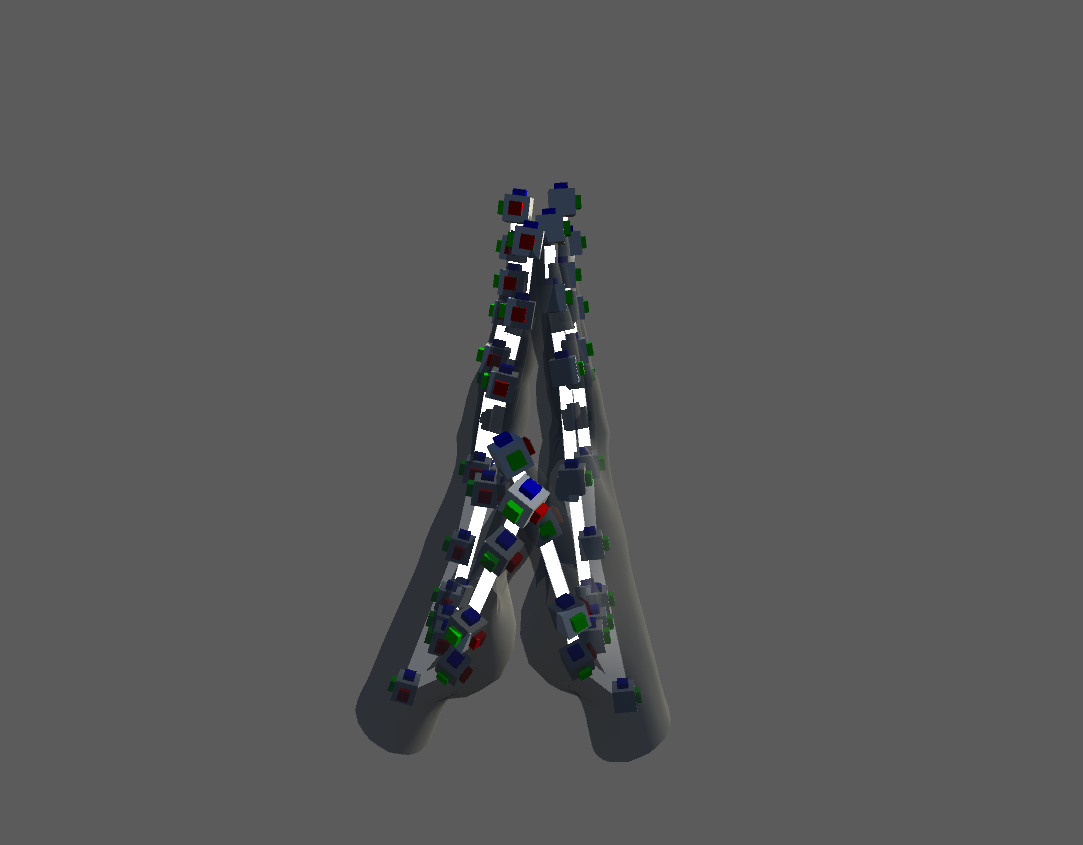
\includegraphics[width=\linewidth]{Clap.png}
    \caption{Clap (Attack)}
    \label{fig:g2hc-clap}
  \end{subfigure}\hfill
  \begin{subfigure}[t]{0.23\textwidth}
    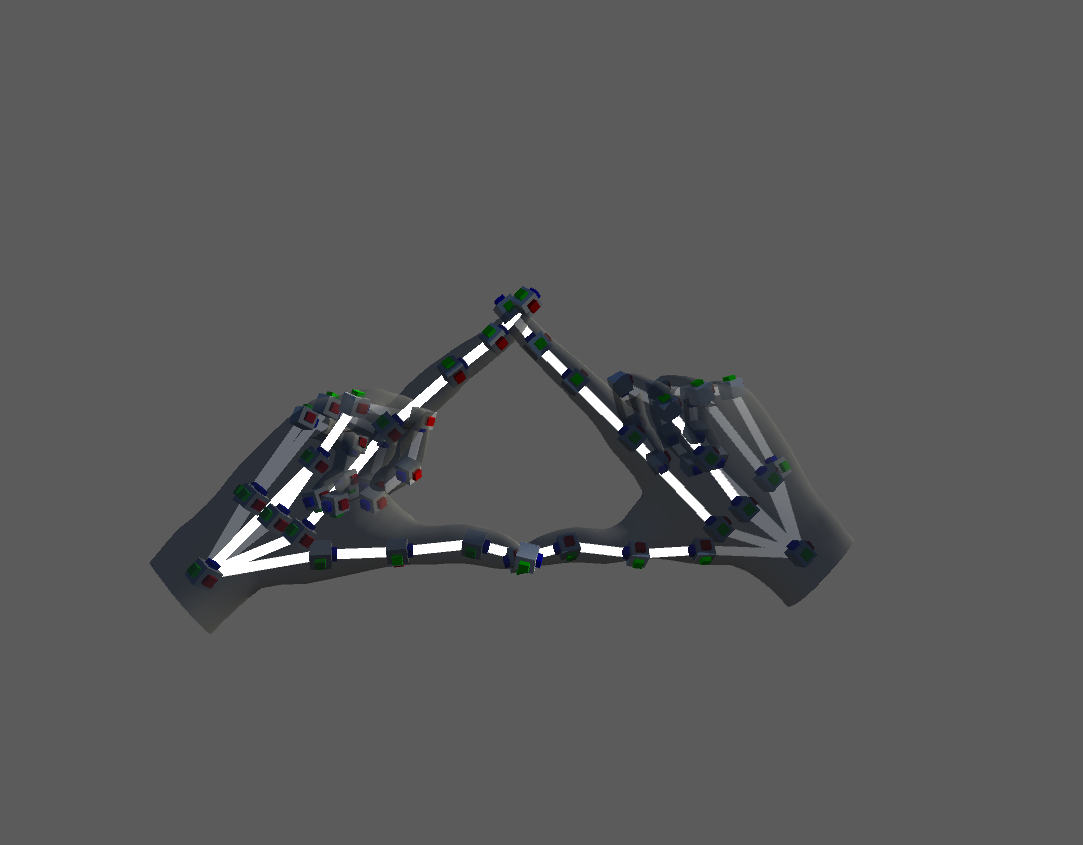
\includegraphics[width=\linewidth]{Triangle.png}
    \caption{Triangle (Defense)}
    \label{fig:g2hc-triangle}
  \end{subfigure}\hfill
  \begin{subfigure}[t]{0.23\textwidth}
    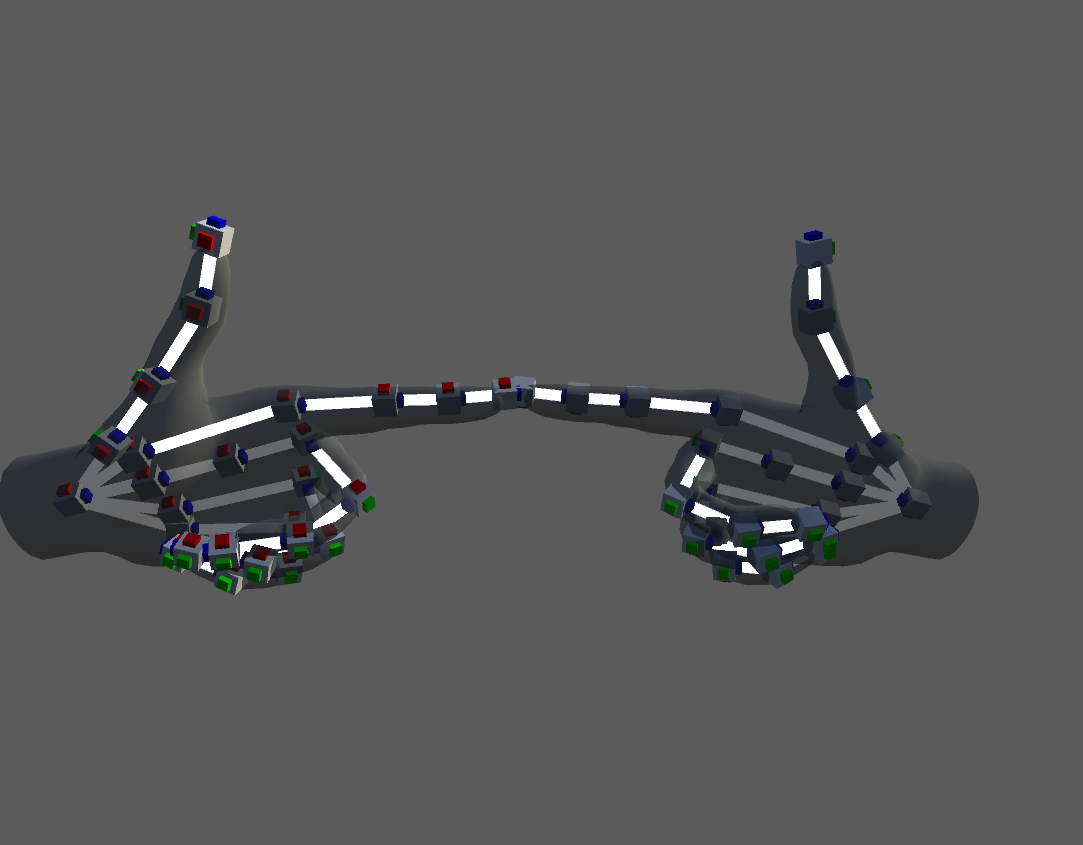
\includegraphics[width=\linewidth]{Cutesy.png}
    \caption{Cutesy (Buff)}
    \label{fig:g2hc-cutesy}
  \end{subfigure}\hfill
  \begin{subfigure}[t]{0.23\textwidth}
    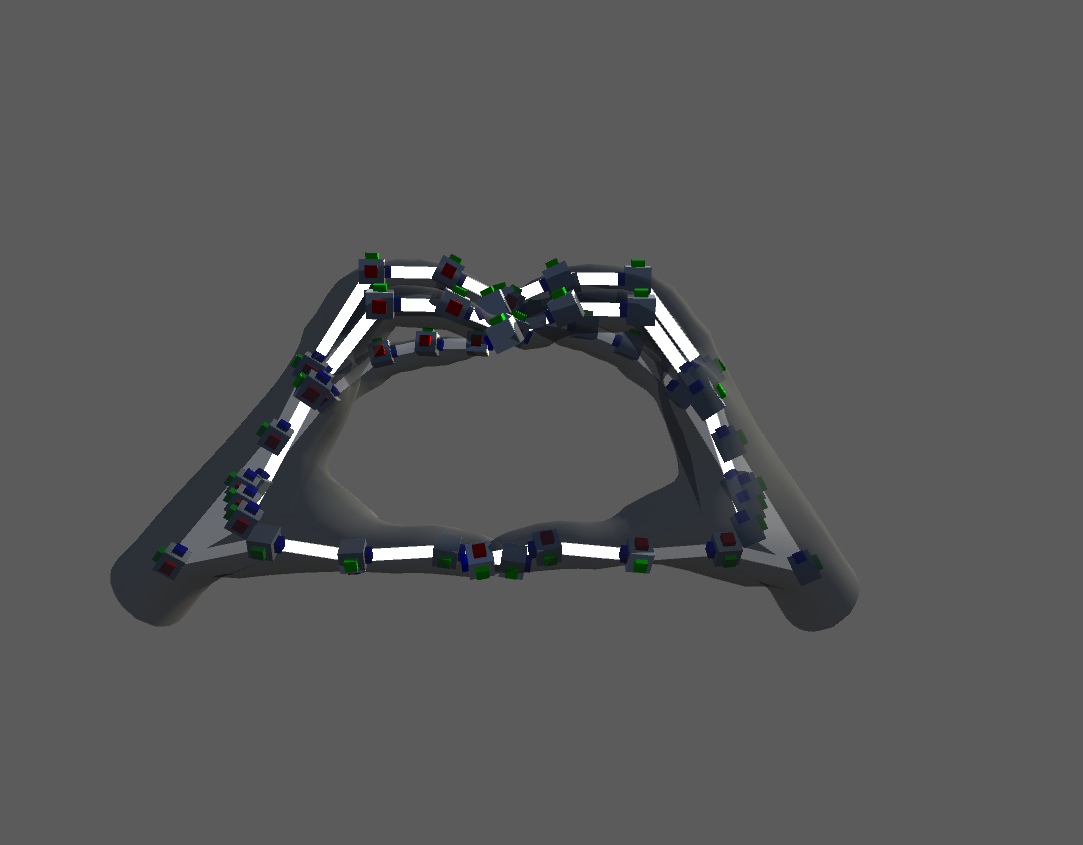
\includegraphics[width=\linewidth]{Heart Hands.png}
    \caption{Heart Hands (Health)}
    \label{fig:g2hc-heart}
  \end{subfigure}
  \caption{Gesture–glyph mappings for the two‐handed combined gesture condition (G2H-C).}
  \label{fig:g2hc-collage}
\end{figure}

\begin{table}[ht]
  \centering
  \caption{Glyph–Gesture mappings for Gesture Two‐Handed Combined (G2H‐C)}
  \label{tab:G2HC-mappings}
  \begin{tabular}{@{}ll@{}}
    \toprule
    \multicolumn{2}{c}{\textbf{Gesture Two‐Handed Combined (G2H‐C)}}\\
    \midrule
    \textbf{Glyph} & \textbf{Gesture} \\
    \midrule
    Attack   & Clap          \\
    Defense  & Triangle      \\
    Buff     & Cutesy        \\
    Health   & Heart Hands   \\
    \bottomrule
  \end{tabular}
\end{table}



\subsection{Efficiency (Time Measures)}
\begin{itemize}
  \item \textbf{Tutorial Time:} mean ± SD per control type; ANOVA results (F, p, η²); post-hoc differences.
  \item \textbf{Glyph‐Creation Time:} same stats.
  \item \textbf{Lesson Completion Time:} same stats.
\end{itemize}
Include a table (or figure) of mean times and error bars, plus a brief sentence summarizing the key differences (e.g.\ “Gesture–Combined was significantly slower than all other methods, p<.001”).

\subsection{Effectiveness (Accuracy Measures)}
\begin{itemize}
  \item \textbf{Tutorial Accuracy:} proportion correct in tutorial lessons; ANOVA or non-parametric test.
  \item \textbf{Glyph Accuracy:} accuracy drawing individual glyphs.
  \item \textbf{Final Lesson Accuracy:} overall spell success rate.
\end{itemize}
Report mean accuracy (± SD), test stats, and note any trends or significant contrasts.

\subsection{Subjective Preference}
\begin{itemize}
  \item Describe the 1–5 preference scale (1 = favorite, 5 = least favorite).
  \item ANOVA on preference ratings, plus post-hoc LSD/Tukey.
  \item Highlight which control types differed (e.g.\ one-handed gesture rated best, combined gesture worst).
\end{itemize}
You can include the “Connecting Letters” or a small bar chart with significance asterisks here.

\subsection{Summary}
One paragraph tying it all together:
\begin{itemize}
  \item Which input was fastest vs.\ most accurate vs.\ most liked?
  \item Any clear trade-offs (e.g.\ fastest ≠ most preferred)?
\end{itemize}


% A formula that appears in the running text is called an inline or
% in-text formula.  It is produced by the \textbf{math} environment,
% which can be invoked with the usual
% \texttt{{\char'134}begin\,\ldots{\char'134}end} construction or with
% the short form \texttt{\$\,\ldots\$}. You can use any of the symbols
% and structures, from $\alpha$ to $\omega$, available in
% \LaTeX~\cite{Lamport:LaTeX}; this section will simply show a few
% examples of in-text equations in context. Notice how this equation:
% \begin{math}
%   \lim_{n\rightarrow \infty}x=0
% \end{math},
% set here in in-line math style, looks slightly different when
% set in display style.  (See next section).

% \subsection{Display Equations}
% A numbered display equation---one set off by vertical space from the
% text and centered horizontally---is produced by the \textbf{equation}
% environment. An unnumbered display equation is produced by the
% \textbf{displaymath} environment.

% Again, in either environment, you can use any of the symbols and
% structures available in \LaTeX\@; this section will just give a couple
% of examples of display equations in context.  First, consider the
% equation, shown as an inline equation above:
% \begin{equation}
%   \lim_{n\rightarrow \infty}x=0
% \end{equation}
% Notice how it is formatted somewhat differently in
% the \textbf{displaymath}
% environment.  Now, we'll enter an unnumbered equation:
% \begin{displaymath}
%   \sum_{i=0}^{\infty} x + 1
% \end{displaymath}
% and follow it with another numbered equation:
% \begin{equation}
%   \sum_{i=0}^{\infty}x_i=\int_{0}^{\pi+2} f
% \end{equation}
% just to demonstrate \LaTeX's able handling of numbering.

% \section{Figures}

% The ``\verb|figure|'' environment should be used for figures. One or
% more images can be placed within a figure. If your figure contains
% third-party material, you must clearly identify it as such, as shown
% in the example below.
% \begin{figure}[h]
%   \centering
%   \includegraphics[width=\linewidth]{sample-franklin}
%   \caption{1907 Franklin Model D roadster. Photograph by Harris \&
%     Ewing, Inc. [Public domain], via Wikimedia
%     Commons. (\url{https://goo.gl/VLCRBB}).}
%   \Description{A woman and a girl in white dresses sit in an open car.}
% \end{figure}

% Your figures should contain a caption which describes the figure to
% the reader.

% Figure captions are placed {\itshape below} the figure.

% Every figure should also have a figure description unless it is purely
% decorative. These descriptions convey what’s in the image to someone
% who cannot see it. They are also used by search engine crawlers for
% indexing images, and when images cannot be loaded.

% A figure description must be unformatted plain text less than 2000
% characters long (including spaces).  {\bfseries Figure descriptions
%   should not repeat the figure caption – their purpose is to capture
%   important information that is not already provided in the caption or
%   the main text of the paper.} For figures that convey important and
% complex new information, a short text description may not be
% adequate. More complex alternative descriptions can be placed in an
% appendix and referenced in a short figure description. For example,
% provide a data table capturing the information in a bar chart, or a
% structured list representing a graph.  For additional information
% regarding how best to write figure descriptions and why doing this is
% so important, please see
% \url{https://www.acm.org/publications/taps/describing-figures/}.

% \subsection{The ``Teaser Figure''}

% A ``teaser figure'' is an image, or set of images in one figure, that
% are placed after all author and affiliation information, and before
% the body of the article, spanning the page. If you wish to have such a
% figure in your article, place the command immediately before the
% \verb|\maketitle| command:
% \begin{verbatim}
%   \begin{teaserfigure}
%     \includegraphics[width=\textwidth]{sampleteaser}
%     \caption{figure caption}
%     \Description{figure description}
%   \end{teaserfigure}
% \end{verbatim}

\section{Citations and Bibliographies}

\bibliographystyle{IEEEtran}
\bibliography{references}

% \section{Acknowledgments}

% Identification of funding sources and other support, and thanks to
% individuals and groups that assisted in the research and the
% preparation of the work should be included in an acknowledgment
% section, which is placed just before the reference section in your
% document.

% This section has a special environment:
% \begin{verbatim}
%   \begin{acks}
%   ...
%   \end{acks}
% \end{verbatim}
% so that the information contained therein can be more easily collected
% during the article metadata extraction phase, and to ensure
% consistency in the spelling of the section heading.

% Authors should not prepare this section as a numbered or unnumbered {\verb|\section|}; please use the ``{\verb|acks|}'' environment.

% \section{Appendices}

% If your work needs an appendix, add it before the
% ``\verb|\end{document}|'' command at the conclusion of your source
% document.

% Start the appendix with the ``\verb|appendix|'' command:
% \begin{verbatim}
%   \appendix
% \end{verbatim}
% and note that in the appendix, sections are lettered, not
% numbered. This document has two appendices, demonstrating the section
% and subsection identification method.

% \section{Multi-language papers}

% Papers may be written in languages other than English or include
% titles, subtitles, keywords and abstracts in different languages (as a
% rule, a paper in a language other than English should include an
% English title and an English abstract).  Use \verb|language=...| for
% every language used in the paper.  The last language indicated is the
% main language of the paper.  For example, a French paper with
% additional titles and abstracts in English and German may start with
% the following command
% \begin{verbatim}
% \documentclass[sigconf, language=english, language=german,
%                language=french]{acmart}
% \end{verbatim}

% The title, subtitle, keywords and abstract will be typeset in the main
% language of the paper.  The commands \verb|\translatedXXX|, \verb|XXX|
% begin title, subtitle and keywords, can be used to set these elements
% in the other languages.  The environment \verb|translatedabstract| is
% used to set the translation of the abstract.  These commands and
% environment have a mandatory first argument: the language of the
% second argument.  See \verb|sample-sigconf-i13n.tex| file for examples
% of their usage.

% \section{SIGCHI Extended Abstracts}

% The ``\verb|sigchi-a|'' template style (available only in \LaTeX\ and
% not in Word) produces a landscape-orientation formatted article, with
% a wide left margin. Three environments are available for use with the
% ``\verb|sigchi-a|'' template style, and produce formatted output in
% the margin:
% \begin{description}
% \item[\texttt{sidebar}:]  Place formatted text in the margin.
% \item[\texttt{marginfigure}:] Place a figure in the margin.
% \item[\texttt{margintable}:] Place a table in the margin.
% \end{description}

% %%
% %% The acknowledgments section is defined using the "acks" environment
% %% (and NOT an unnumbered section). This ensures the proper
% %% identification of the section in the article metadata, and the
% %% consistent spelling of the heading.
% \begin{acks}
% To Robert, for the bagels and explaining CMYK and color spaces.
% \end{acks}

% %%
% %% The next two lines define the bibliography style to be used, and
% %% the bibliography file.
% \bibliographystyle{ACM-Reference-Format}
% \bibliography{sample-base}


% %%
% %% If your work has an appendix, this is the place to put it.
% \appendix

% \section{Research Methods}

% \subsection{Part One}

% Lorem ipsum dolor sit amet, consectetur adipiscing elit. Morbi
% malesuada, quam in pulvinar varius, metus nunc fermentum urna, id
% sollicitudin purus odio sit amet enim. Aliquam ullamcorper eu ipsum
% vel mollis. Curabitur quis dictum nisl. Phasellus vel semper risus, et
% lacinia dolor. Integer ultricies commodo sem nec semper.

% \subsection{Part Two}

% Etiam commodo feugiat nisl pulvinar pellentesque. Etiam auctor sodales
% ligula, non varius nibh pulvinar semper. Suspendisse nec lectus non
% ipsum convallis congue hendrerit vitae sapien. Donec at laoreet
% eros. Vivamus non purus placerat, scelerisque diam eu, cursus
% ante. Etiam aliquam tortor auctor efficitur mattis.

% \section{Online Resources}

% Nam id fermentum dui. Suspendisse sagittis tortor a nulla mollis, in
% pulvinar ex pretium. Sed interdum orci quis metus euismod, et sagittis
% enim maximus. Vestibulum gravida massa ut felis suscipit
% congue. Quisque mattis elit a risus ultrices commodo venenatis eget
% dui. Etiam sagittis eleifend elementum.

% Nam interdum magna at lectus dignissim, ac dignissim lorem
% rhoncus. Maecenas eu arcu ac neque placerat aliquam. Nunc pulvinar
% massa et mattis lacinia.

\end{document}
\endinput
%%
%% End of file `sample-acmlarge.tex'.
